\documentclass[../../../../main.tex]{subfiles}
\begin{document}

\begin{flushright}
\footnotesize\textit{【自動文字起こし・要確認】}
\end{flushright}

[解] $a,b,c>0 \cdots$ \textcircled{1}
\begin{equation*}
\pi : \frac{x}{a} + \frac{y}{b} + \frac{z}{c} = 0 \cdots \textcircled{2}
\end{equation*}

\textcircled{2}の表式から、$\pi$は3点$(0,0,0)$、$(a,-b,0)$、$(0,b,-c)$を通る平面で、切り口は右のような六角形になる。従って、
$AD, AF, DE, BC, BF, CE$
との交点
\begin{align*}
AD &: z=0, y=x-1 \text{ より交点 } \left(\frac{a}{a+b}, \frac{-b}{a+b}, 0\right) \\
AF &: y=0, z=x-1 \text{ より交点 } \left(\frac{a}{a+c}, 0, \frac{-c}{a+c}\right) \\
DE &: x=0, z=y+1 \text{ より交点 } \left(0, \frac{-b}{b+c}, \frac{c}{b+c}\right) \\
BC &: z=0, y=x+1 \text{ より交点 } \left(\frac{-a}{a+b}, \frac{b}{a+b}, 0\right) \\
BF &: x=0, z=y-1 \text{ より交点 } \left(0, \frac{a}{b+c}, \frac{-c}{b+c}\right) \\
CE &: y=0, x=z+1 \text{ より交点 } \left(\frac{-a}{a+c}, 0, \frac{c}{a+c}\right)
\end{align*}

\begin{center}
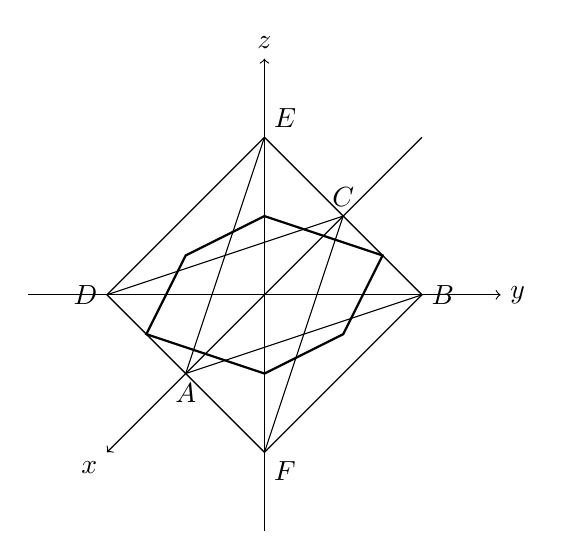
\begin{tikzpicture}[scale=2]
% Draw coordinate axes
\draw[->] (-1.5,0) -- (1.5,0) node[right] {$y$};
\draw[->] (0,-1.5) -- (0,1.5) node[above] {$z$};
\draw[->] (1,1) -- (-1,-1) node[below left] {$x$};
% Draw octahedron vertices
\coordinate (A) at (-0.5,-0.5); % x=1
\coordinate (C) at (0.5,0.5);   % x=-1
\coordinate (B) at (1,0);       % y=1
\coordinate (D) at (-1,0);      % y=-1
\coordinate (E) at (0,1);       % z=1
\coordinate (F) at (0,-1);      % z=-1

% Draw edges
\draw (A) node[below] {$A$} -- (B) node[right] {$B$} -- (C) node[above] {$C$} -- (D) node[left] {$D$} -- cycle;
\draw (E) node[above right] {$E$} -- (A);
\draw (E) -- (B);
\draw (E) -- (C);
\draw (E) -- (D);
\draw (F) node[below right] {$F$} -- (A);
\draw (F) -- (B);
\draw (F) -- (C);
\draw (F) -- (D);

% Draw plane cutting it
\draw[thick] (-0.75,-0.25) -- (0,-0.5) -- (0.5,-0.25) -- (0.75,0.25) -- (0,0.5) -- (-0.5,0.25) -- cycle;
\end{tikzpicture}
\end{center}

\end{document}
